\input{../.preambles/00-lectures}
\input{../.preambles/10-russian}
\input{../.preambles/20-math}

\newcommand{\header}[1]{\vspace*{.3em}\emph{#1}\vspace*{.2em}}
\newcommand{\Der}[2]{\frac{\Delta #1}{\Delta #2}}
\newcommand{\defeq}{\stackrel{\mathrm{def}}{=}}
\newcommand{\D}{\,\Delta}

\begin{document}
\emph{1. Способы задания движения материальной точки. Векторный и координатный
способы задания движения. Определение траектории движения, скорости, ускорения.}

\vspace*{1em}
Существует три способа задания движения точки: естественный, векторный и
координатный. Остановимся на двух последних.

\header{Векторный способ задания движения}
\begin{table}[h!]
    \begin{tabular}{C{.4}m{.55\textwidth}}
        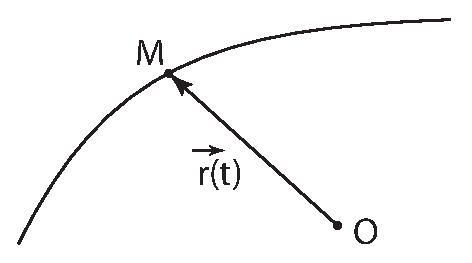
\includegraphics[width=.4\textwidth]{1_vect} &
        Положение точки в пространстве однозначно определяется заданием
        радиус-вектора \( \vec{r} \), проведенного из некоторого неподвижного
        центра \( O \) в данную точку \( M \).
        
        Для определения движения точки нужно знать как меняется с течением
        времени радиус-вектор \( \vec{r} \), то есть должна быть задана
        вектор-функция
    \end{tabular}
\end{table}

аргумента \( t \):
\[
    \vec{r} = \vec{r}(t).
\]

Траектория движения представляет собой геометрическое место концов
радиус-вектора \( \vec{r} \) движущейся точки.

\header{Координатный способ задания движения}

Рассмотрим движение точки \( M \) в трехмерном пространстве. Введем
прямоугольные декартовы координаты \( Oxyz \). Тогда в системе отсчета
\( Oxyz \) положение точки \( M \) определяется тремя координатами
\( (x, y, z) \). При движении точки \( M \) ее координаты изменяются с течением
времени. Следовательно:
\[ \left\{ \begin{array}{l}
    x = f_1(t); \\
    y = f_2(t); \\
    z = f_3(t).
\end{array} \right. \]

Эти уравнения называются уравнениями движения точки в декартовых координатах. Их
можно рассматривать как параметрические уравнения траектории точки. При
исключении параметра \( t \) из уравнений движения получаются уравнения
траектории в координатной форме.

Так, решив первое уравнение относительно \( t \), получим \( t = \phi(x) \).
Подставив полученное выражение для \( t \) в два других уравнения, получаем
уравнения траектории точки в координатной форме:
\[ \left\{ \begin{array}{l}
    x = f_1[\phi(x)]; \\
    y = f_2[\phi(x)].
\end{array} \right. \]
Координатный способ может быть получен из векторного проецированием на орты, так
как имеет место представление радиус-вектора:
\[
    \vec{r}(t) = x(t)\cdot\vec{e}_x + y(t)\cdot\vec{e}_y + z(t)\cdot\vec{e}_z.
\]

\header{Скорость}

Скорость -- это векторная величина, характеризующая быстроту и направление
движения точки в данной системе отсчета. При векторном способе задания движения
скорость:
\[
    \vec{v} \defeq \lim_{\D t \to 0} \Der{\vec{r}}{t} = \der{\vec{r}}{t}.
\]

Из определения следует, что скорость является производной по времени от радиус
вектора и направлена по касательной к траектории в сторону движения точки.

Для координатного способа получим (в декартовых координатах):
\[
    \vec{v} = \der{\vec{r}}{t} = \der{}{t}\Big(x(t)\cdot\vec{e}_x +
    y(t)\cdot\vec{e}_y + z(t)\cdot\vec{e}_z\Big) = \der{x}{t}\cdot\vec{e}_x +
    \der{y}{t}\cdot\vec{e}_y + \der{z}{t}\cdot\vec{e}_z = v_x\cdot\vec{e}_x +
    v_y\cdot\vec{e}_y + v_z\cdot\vec{e}_z.
\]

Следовательно, проекции скорости точки на неподвижные оси декартовых координат
равны первым производным от соответствующих координат точки по времени.

Модуль скорости и её направление можно определить, зная проекции:
\[
    v = \sqrt{v_x^2 + v_y^2 + v_z^2}, \quad
    \cos\left(\vec{v}, \vec{e}_x\right) = \frac{v_x}{v},\ \ 
    \cos\left(\vec{v}, \vec{e}_y\right) = \frac{v_y}{v},\ \ 
    \cos\left(\vec{v}, \vec{e}_z\right) = \frac{v_z}{v}.
\]

\header{Ускорение}

При неравномерном криволинейном движении точки изменяются модуль и направление
её скорости. Ускорение точки характеризует быстроту изменения модуля и
направления скорости точки.
\[
    \vec{a} \defeq \lim_{\D t \to 0} \Der{\vec{v}}{t} = \der{\vec{v}}{t} =
    \dder{\vec{r}}{t}.
\]

Вектор ускорения направлен по касательной к годографу скорости, расположен в
соприкасающейся плоскости и направле в сторону вогнутости кривой.

Как и в случае со скоростью, можно перейти к координатам. Получим:
\begin{align*}
    a_x = \dder{x}{t},\ \ a_y & = \dder{y}{t},\ \ a_z = \dder{z}{t}; \\
    a = \sqrt{a_x^2 + a_y^2 + a_z^2}, \quad
    \cos\left(\vec{a}, \vec{e}_x\right) = \frac{a_x}{a}, & \ \ 
    \cos\left(\vec{a}, \vec{e}_y\right) = \frac{a_y}{a},\ \ 
    \cos\left(\vec{a}, \vec{e}_z\right) = \frac{a_z}{a}.
\end{align*}

\newpage % ---------------------------------------------------------------------

\emph{2. Общее уравнение динамики (принцип Д'Аламбера-Лагранжа).}

\newpage % -------------------------------------------------------------------

\emph{3. Общее уравнение динамики в обобщенных координатах. Уравнения Лагранжа
2-го рода. Примеры применения уравнений Лагранжа в потенциальном поле сил.}

\newpage % ---------------------------------------------------------------------

\emph{4. Параллельное векторное поле. Символы Кристофеля первого и второго
рода. Определение символов Кристофеля через фундаментальный метрический тензор.}

\newpage % ---------------------------------------------------------------------

\emph{5. Понятие об абсолютной и ковариантной производных.}

\newpage % ---------------------------------------------------------------------

\emph{6. Естественный способ задания движения. Определение скорости и ускорения
точки. Нормальное, касательное ускорения. Их физический смысл. Определение
касательного и нормального ускорений при координатном способе задания движения.}



\newpage % ---------------------------------------------------------------------

\emph{7. Уравнения Лагранжа 1-го рода. Понятие об избыточных координатах.
Неопределенные множители Лагранжа. Полная система уравнений, описывающая
движение механической системы с избыточными координатами. Примеры применения.}

\newpage % ---------------------------------------------------------------------

\emph{8. Переменные Лагранжа и Эйлера для описания движения частицы сплошной
среды. Вектор смещения. Тензор смещения как сумма тензора деформации и тензора
поворота.}

\newpage % ---------------------------------------------------------------------

\emph{9. Основные законы динамики материальной точки. Законы Ньютона.
Дифференциальные уравнения движения материальной точки. Две основные задачи
динамики точки.}

\newpage % ---------------------------------------------------------------------

\emph{10. Понятие об изохронной и полной вариациях функции. Действие по
Гамильтону. Принцип наименьшего действия Гамильтона-Остроградского.}

\newpage % ---------------------------------------------------------------------

\emph{11. Физический смысл дивергенции вектора смещения. Понятие о тензоре
скоростей деформации.}

\newpage % ---------------------------------------------------------------------

\emph{12. Основные законы (теоремы) механики для материальной точки. Закон
сохранения импульса. Теорема об изменении количества движения.}

\newpage % ---------------------------------------------------------------------

\emph{13. Принцип наименьшего действия Монертюн-Лагранжа. Действие по Лагранжу.}

\newpage % ---------------------------------------------------------------------

\emph{14. Принцип наименьшего действия Монертюн-Лагранжа в форме Якоби.}

\newpage % ---------------------------------------------------------------------

\emph{15. Кинетический момент твердого тела относительно неподвижной точки.
Кинетическая энергия твердого тела, совершающего сферическое движение.
Динамические уравнения Эйлера.}

\newpage % ---------------------------------------------------------------------

\emph{16. Основные законы (теоремы) механики для материальной точки. Теорема об
изменении момента импульса (момента количества движения, кинетического
момента). Закон сохранения момента импульса.}

\newpage % ---------------------------------------------------------------------

\emph{17. Функция Гамильтона. Канонические уравнения Гамильтона. Примеры
применения уравнений Гамильтона.}

\newpage % ---------------------------------------------------------------------

\emph{18. Основные законы (теоремы) механики для материальной точки. Теорема об
изменении кинетической энергии. Закон сохранения механической энергии.}

\newpage % ---------------------------------------------------------------------

\emph{19. Циклические координаты и циклические интегралы. Связь циклических
интегралов с законами сохранения.}

\newpage % ---------------------------------------------------------------------

\emph{20. Структура кинетической энергии в обобщенных координатах. Матрица
инерционных коэффициентов уравнений Лагранжа в случае стационарных связей.}

\newpage % ---------------------------------------------------------------------

\emph{21. Полная система уравнений, описывающая движение частицы сплошной
среды. Уравнение состояния. Простейшие модели сплошных сред: линейное
упругое тело, идеальная жидкость.}

\newpage % ---------------------------------------------------------------------

\emph{22. Определение скорости и ускорения точки в полярной системе координат.
Дифференциальные уравнения движения материальной точки в цилиндрической
системе координат. Количество движения, кинетический момент и кинетическая
энергия материальной точки в цилиндрической системе координат.}

\newpage % ---------------------------------------------------------------------

\emph{23. Кинематика твердого тела. Равновесие твердого тела.}

\newpage % ---------------------------------------------------------------------

\emph{24. Кинематика твердого тела. Поступательное движение.}

\newpage % ---------------------------------------------------------------------

\emph{25. Кинематика твердого тела. Вращательное движение вокруг неподвижной
оси.}

\newpage % ---------------------------------------------------------------------

\emph{26. Кинематика твердого тела. Плоское движение. Определение кинематических
характеристик движения: траектории движения скорости и ускорения
произвольной точки тела. Понятие о мгновенном центре скоростей.}

\newpage % ---------------------------------------------------------------------

\emph{27. Исследование движения материальной точки в центрально-симметричном
поле сил. Первые интегралы уравнений движения. Понятие об эффективной
потенциальной энергии. Интегрирование уравнений движения.}

\newpage % ---------------------------------------------------------------------

\emph{28. Принцип возможных перемещений (принцип Лагранжа). Доказательство
необходимости и достаточности. Примеры применения принципа возможных
перемещений.}

\newpage % ---------------------------------------------------------------------

\emph{29. Массово-геометрические характеристики твердого тела. Моменты инерции
относительно точки, оси. Центробежные моменты инерции. Теорема
Гюйгенса-Штейнера. Вычисление моментов инерции тела относительно оси
заданного направления.}

\newpage % ---------------------------------------------------------------------

\emph{30. Дифференциальное уравнение поступательного движения частицы сплошной
среды. Ковариантная форма уравнения движения. Движение частицы сплошной
среды относительно ее центра масс. Закон парности касательных напряжении.}

\newpage % ---------------------------------------------------------------------

\emph{31. Движение материальной точки в неинерциальной системе координат.
Абсолютное, переносное и относительное движение. Понятие об абсолютной
(полной) и местной (локальной) производных. Формула Бура. Определение
абсолютной скорости и ускорения материальной точки. Кориолисово ускорение.}

\newpage % ---------------------------------------------------------------------

\emph{32. Сферическое движение твердого тела. Уравнения движения. Углы Эйлера.
Определение скорости произвольной точки твердого тела. Кинематические
уравнения Эйлера. Уравнение мгновенной оси вращения.}

\newpage % ---------------------------------------------------------------------

\emph{33. Преобразование координат. Понятие тензора. Ковариантные и
контрвариантные компоненты вектора, тензора. Криволинейные координаты.
Фундаментальный метрический тензор.}

\newpage % ---------------------------------------------------------------------

\emph{34. Динамика относительного движения материальной точки. Переносная и
кориолисова силы инерции. Принцип относительности Галилея. Частные случаи
движения.}

\newpage % ---------------------------------------------------------------------

\emph{35. Обобщенные силы. Способы вычисления обобщенных сил. Понятие об
идеальных связях. Вычисление обобщенных сил в случае движения механической
системы в поле потенциальных сил.}

\newpage % ---------------------------------------------------------------------

\emph{36. Параллельное векторное поле. Символы Кристофеля первого и второго
рода. Определение символов Кристофеля через фундаментальный метрический
тензор. Понятие об абсолютной и ковариантной производных.}

\newpage % ---------------------------------------------------------------------

\emph{37. Понятие об обобщенных координатах. Понятие о связях. Классификация
связей. Возможные (виртуальные) перемещения. Число степеней свободы
механической системы.}

\newpage % ---------------------------------------------------------------------

\emph{38. Кинетическая энергия механической системы. Теорема Кенига. Теорема об
изменении кинетической энергии механической системы. Закон сохранения
полной механической энергии.}

\newpage % ---------------------------------------------------------------------

\emph{39. Уравнение неразрывности. Вид уравнения неразрывности в декартовой и
криволинейных координатах.}

\newpage % ---------------------------------------------------------------------

\emph{40. Понятие механической системы. Основные характеристики механической
системы: масса, центр масс. Внутренние силы и их свойства. Дифференциальные
уравнения движения механической системы. Теорема о движении центра масс
механической системы. Закон сохранения движения центра масс.}

\newpage % ---------------------------------------------------------------------

\emph{41. Определение траектории движения материальной точки в движущемся
центрально-симметричном поле сил. Дифференциальное уравнение траектории
движения. Уравнение Бине. Решение уравнения Бине. Виды траекторий. Влияние
начальных условий на вид траектории.}

\newpage % ---------------------------------------------------------------------

\emph{42. Сферическое движение твердого тела. Уравнения движения. Углы Эйлера.
Определение скорости произвольной точки твердого тела. Кинематические
уравнения Эйлера. Уравнение мгновенной оси вращения.}

\newpage % ---------------------------------------------------------------------

\emph{43. Механическая система (изменяемая и неизменяемая). Масса системы. Центр
масс и его координаты. Статические моменты массы системы относительно
полюса и плоскости. Статические моменты массы относительно центра масс и
плоскостей, проходящих через центр масс.}

\newpage % ---------------------------------------------------------------------

\emph{44. Классификация сил, действующих на механическую систему: силы внутренние
и внешние, задаваемые силы. Главный вектор и главный момент внутренних сил.
Дифференциальные уравнения движения механической системы.}

\newpage % ---------------------------------------------------------------------

\emph{45. Количество движения точки и системы. Элементарный и полный импульс
силы. Теорема об изменении количества движения точки в дифференциальной и
конечной формах. Теорема импульсов.}

\newpage % ---------------------------------------------------------------------

\emph{46. Количество движения системы и способы его вычисления. Теорема об
изменении количества движения системы в дифференциальной и конечной
формах. Законы сохранения количества движения системы.}

\newpage % ---------------------------------------------------------------------

\emph{47. Теорема о движении центра масс механической системы. Следствия из
теоремы. Дифференциальные уравнения поступательного движения твердого
тела.}

\newpage % ---------------------------------------------------------------------

\emph{48. Кинетический момент точки и системы относительно центра и оси.
Кинетический момент вращающегося твердого тела относительно оси вращения.
Теорема об изменении кинетического момента для точки.}

\newpage % ---------------------------------------------------------------------

\emph{49. Теорема об изменении кинетического момента для механической системы.
Законы сохранения кинетических моментов. Дифференциальное уравнение
вращательного движения твердого тела вокруг неподвижной оси. Физический
маятник.}

\newpage % ---------------------------------------------------------------------

\emph{50. Кинетический момент системы в абсолютном движении. Теорема об
изменении кинетического момента системы в относительном движении по
отношению к центру масс. Дифференциальные уравнения плоского движения
твердого тела.}

\newpage % ---------------------------------------------------------------------

\emph{51. Элементарная работа силы и ее аналитическое выражение. Работа силы на
конечном пути. Работа равнодействующей. Мощность.}

\newpage % ---------------------------------------------------------------------

\emph{52. Примеры вычисления работы силы. Работа силы тяжести, линейной силы
упругости и силы тяготения.}

\newpage % ---------------------------------------------------------------------

\emph{53. Работа и мощность сил. приложенных к твердому телу при поступательном,
вращательном, сферическом и свободном движении твердого тела. Работа
внутренних сил твердого тела.}

\newpage % ---------------------------------------------------------------------

\emph{54. Кинетическая энергия материальной точки и системы. Теорема Кенига.
Кинетическая энергия твердого тела в поступательном, вращательном и плоском
движениях.}

\newpage % ---------------------------------------------------------------------

\emph{55. Теорема об изменении кинетической энергии материальной точки и системы
в дифференциальной и конечной формах. Случай абсолютно твердого тела.}

\end{document}
